\section{Introduction}

\par Morphological parser is a fundamental tool, a wide range of computational linguistics' tasks rely on some form of morphological model. For morphologically rich languages it is close to impossible to list and manually define all the possible word-forms. The only reasonable way to approach such problem is to model a language's morphology. 
\par For high-resource languages morphology modeling is usually approached using deep learning (DL) models, which are trained on large amounts of data. This method is not available for low-resource languages that lack digital textual data, for such languages linguists usually apply rule-based approach. Shughni is a low-resource language with very few data available, which leaves us the rule-based option.
\begin{figure}[!b]
    \centering
    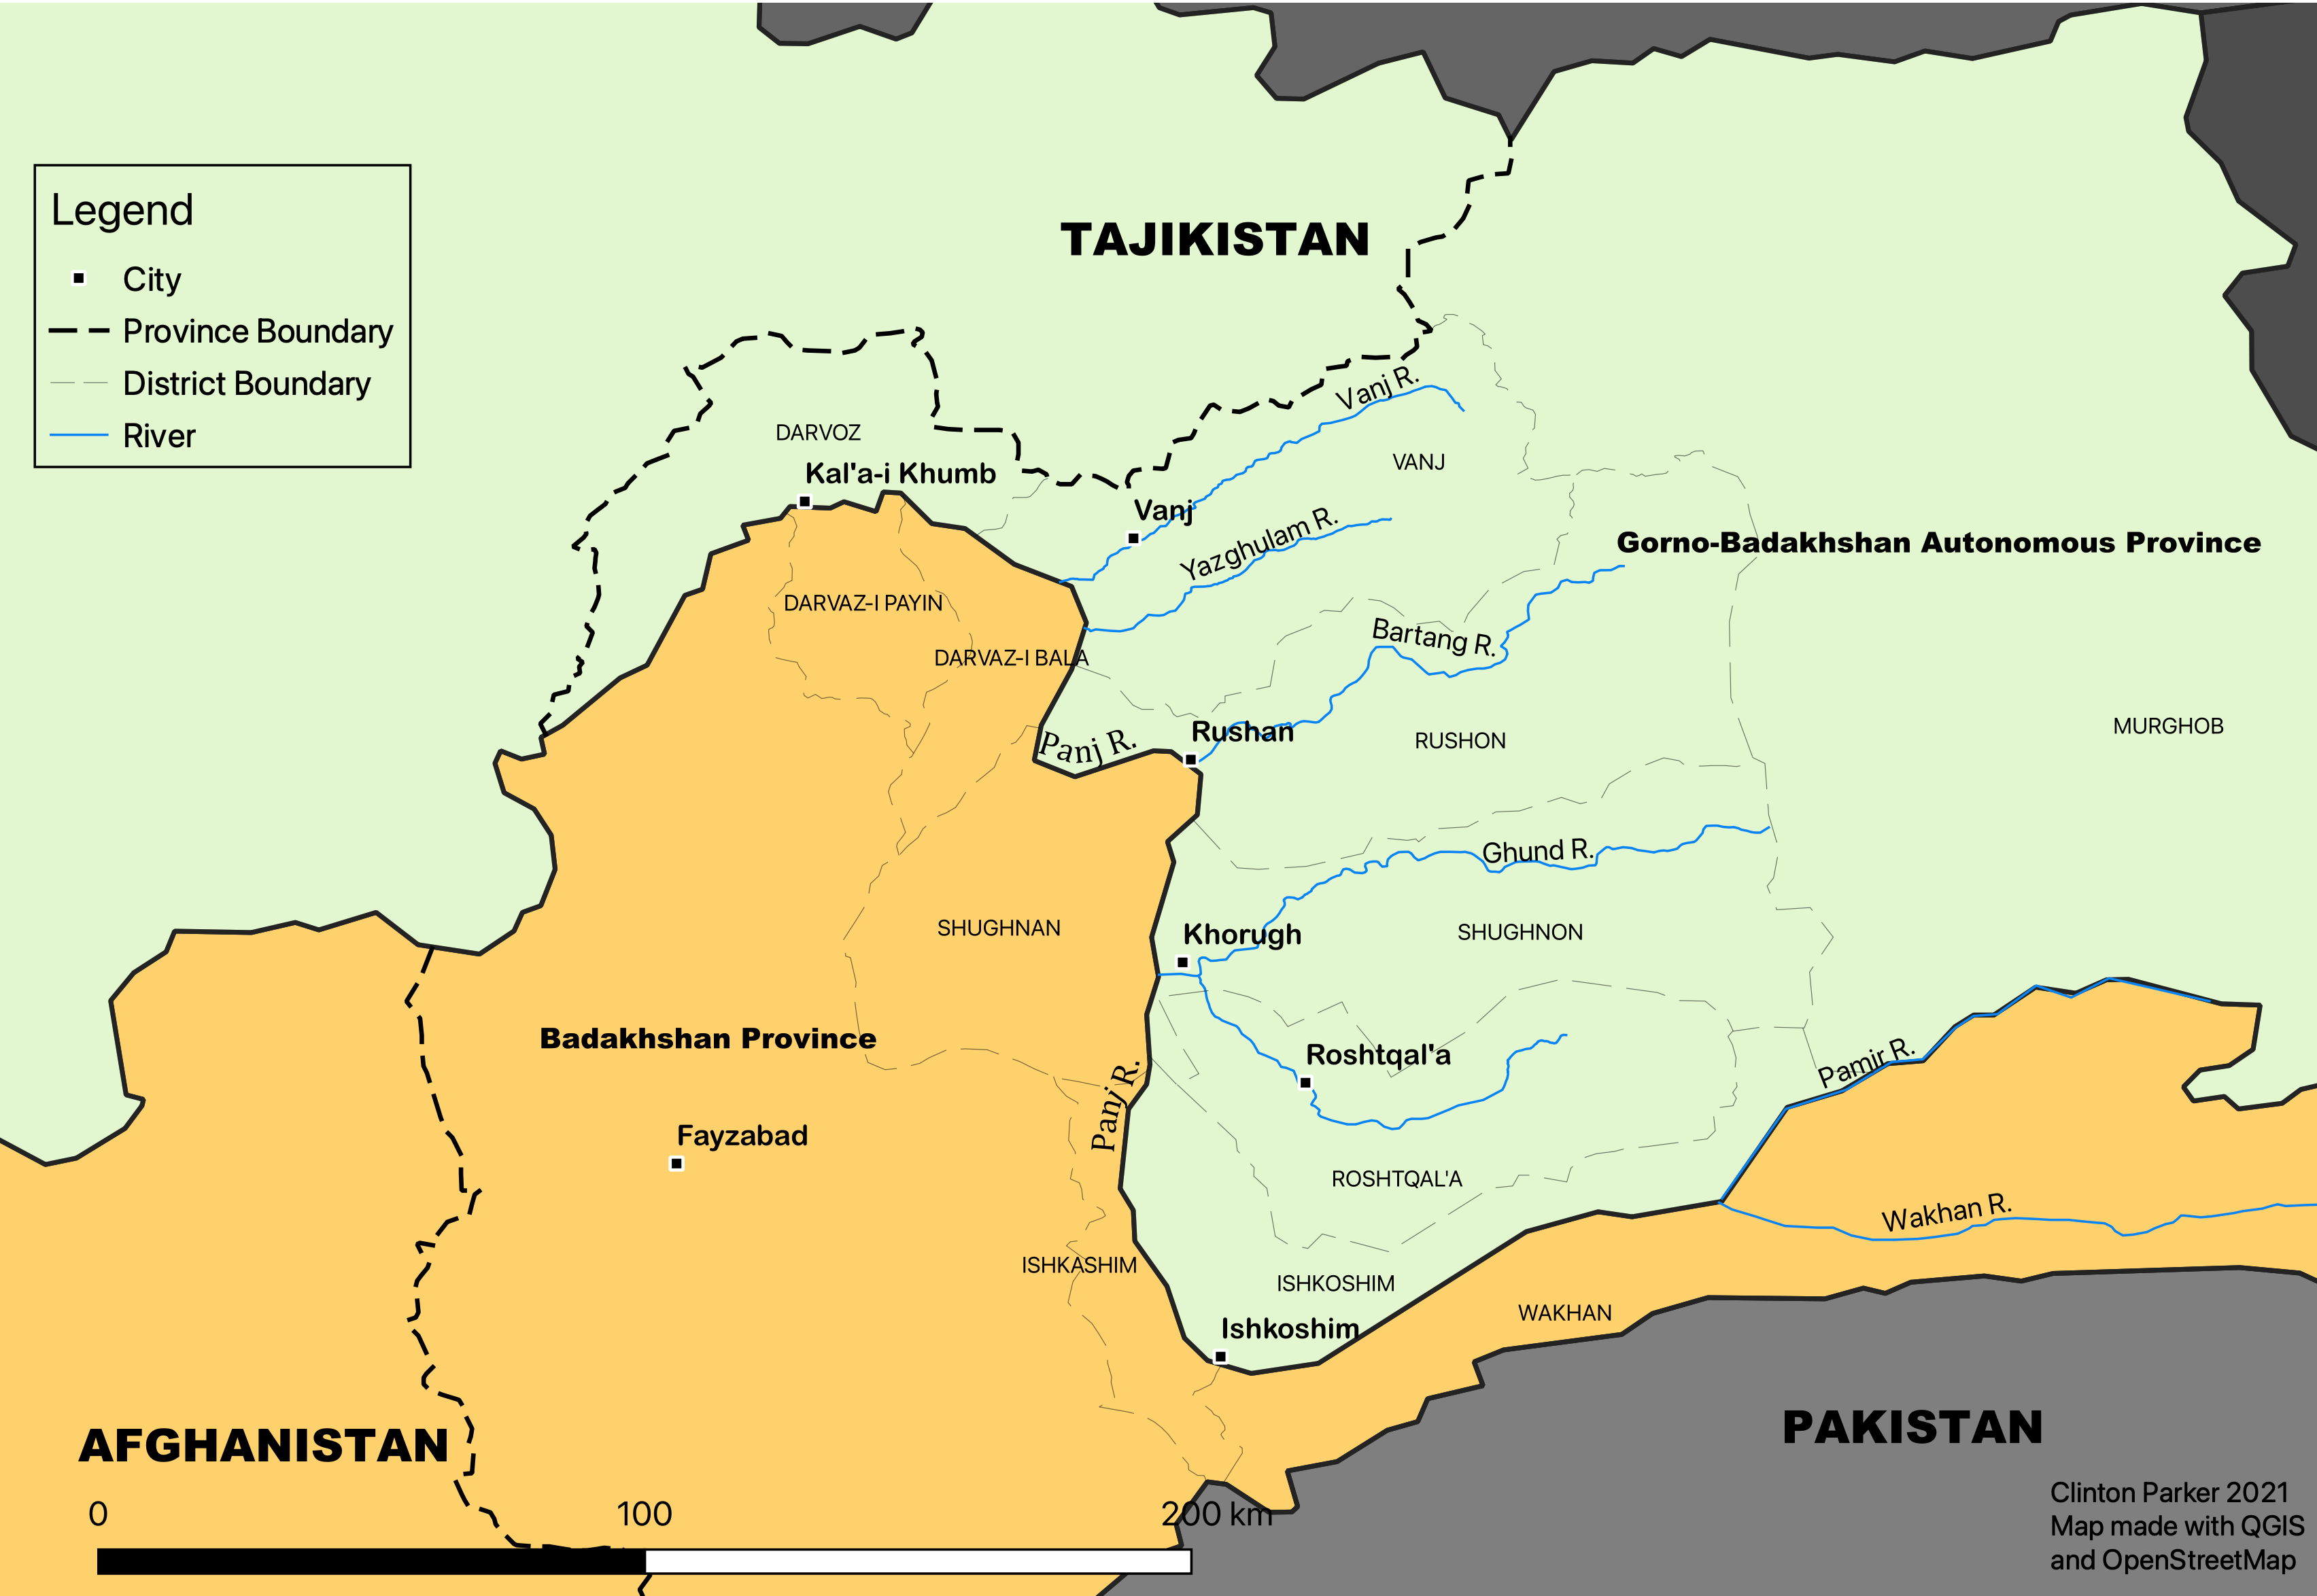
\includegraphics[scale=0.125]{\rootdir/map.png}
    \caption{Mountainous Badakhshan Autonomous Province of Tajikistan and Badakhshan Province of Afghanistan, \parencite[Fig 1.1]{parker_shughni_2023}}
    \label{fig:map1}
\end{figure}
\par Shughni language (ISO: sgh; glottolog: shug1248) is a low-resource language. It belongs to the Iranian branch of the Indo-European family \parencite[12]{plungian_study_2022}, and it is spoken by circa 80 000 - 100 000 people \parencite{edelman_dodykhudoeva_shughni_2009} in two regions: Mountainous Badakhshan Autonomous Region (Tajikistan) and Badakhshan Province (Afghanistan). Both regions have a subregion, where Shughni language is the most spoken native language, the subregions are called 'Shughnon' in Tajikistan and 'Shughnan' in Afghanistan \parencite[2]{parker_shughni_2023}, see Figure \ref{fig:map1} for details. Shughni has a mixed morphological typology type \parencite[94]{parker_shughni_2023}, which means that grammatical meanings can be carried by morphemes, words or clitics. There are three scripts for Shughni language: Latin, Cyrillic and Arabic. The Arabic script is used on the territory of Badakhshan Province of Afghanistan, and Cyrillic and Latin scripts are used in the Mountainous Badakhshan Autonomous Region of Tajikistan. The Cyrillic script was created and gained popularity in 1930s, after it was set as the primary script for teaching in schools on the Shughni-speaking territory of Tajikistan.
\par Morphology analysis tools in question will focus on the variation of Shughni that is spoken in Tajikistan. Cyrillic and Latin script will be supported: the core analysis tool will be implemented in Cyrillic script, and Latin script support will be implemented via transliteration.